\chapter{Methodology}
\clearpage

\section{Introduction}
Automated skin lesion classification enables early and accurate diagnosis of dermatological pathologies. In this study, we develop a robust end-to-end pipeline—from data acquisition and augmentation to model training, evaluation, and edge deployment. Our implementation leverages a Mixture-of-Experts architecture in PyTorch, trained on a platform with an RTX 3060 Lite (12 GB VRAM), 32 GB RAM, and a Ryzen 7 CPU over approximately 76 hours. Future research will explore deployment on Coral Dev Boards with integrated Edge TPUs for advanced, ultra‑low‑latency inference.
%add image for cancers here 
\begin{figure}[h!]
  \centering
  % Placeholder for skin lesion images
  \includegraphics[width=0.7\textwidth]{Untitled.jpg} % Replaced placeholder with actual image
  \caption{Example skin lesion images from the HAM10000/isic 2018 datasets, illustrating the diversity of pathologies including melanoma, basal cell carcinoma, and nevus.}
  \label{fig:skin-lesion-examples}
\end{figure}
\section{Dataset Acquisition and Augmentation}
We utilize the Balanced Skin Cancer MNIST HAM10000 dataset, which augments the original ISIC challenge images to achieve a balanced class distribution. The augmentation pipeline is available at:
\begin{itemize}
\item \url{https://github.com/utkarsh231/Balanced-Skin-Cancer-MNIST-HAM-10000-Dataset}
\end{itemize}
Original sources include:
\begin{itemize}
\item ISIC 2018 Challenge: \url{https://challenge2018.isic-archive.com}
\item HAM10000 on Harvard Dataverse: \url{https://dataverse.harvard.edu/dataset.xhtml?persistentId=doi:10.7910/DVN/DBW86T}
\end{itemize}
This dataset comprises over 39,500 dermoscopic images evenly distributed across seven pathology classes. Foundational studies include Codella \emph{et al.}\cite{codella2018skin} and Tschandl \emph{et al.}\cite{tschandl2018ham10000}. To improve generalization, we apply online data augmentation using Albumentations:

\begin{figure}[h!]
  \centering
  % Placeholder for data augmentation pipeline visualization
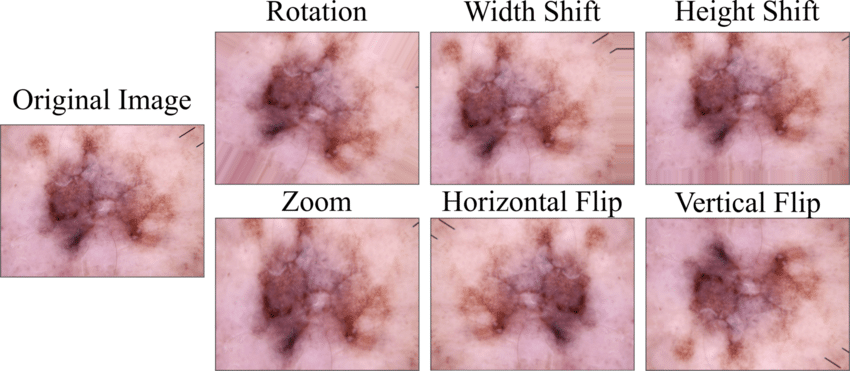
\includegraphics[width=0.8\textwidth]{Data-augmentation.png}
  \caption{Visualization of the data augmentation pipeline applied to a sample image. This figure would illustrate the sequence of transformations such as resizing, random cropping, flips, and color jittering.}
  \label{fig:data-augmentation-pipeline}
\end{figure}

\begin{itemize}
\item \textbf{Resize:} scale images to \texttt{(450, 600)} (height, width)
\item \textbf{RandomResizedCrop:} size=(450, 600), scale=(0.8--1.0)
\item Horizontal and vertical flips ($p=0.5$)
\item Brightness and contrast perturbations ($p=0.3$)
\item Pixel normalization to zero mean and unit variance
\end{itemize}
A custom \texttt{ClassificationDataset} loads images and labels, while a \texttt{WeightedRandomSampler} biases sampling toward under-represented classes.

\section{Model Architecture}
Our Mixture-of-Experts (MoE) framework integrates specialist and generalist feature extractors:

\begin{figure}[h!]
  \centering
  % Placeholder for model architecture diagram
  \fbox{\parbox[c][12cm][c]{0.9\textwidth}{\centering Model Architecture Diagram Placeholder}}
  \caption{High-level architecture of the Mixture-of-Experts (MoE) model. This diagram would show the specialist experts (EfficientNet-b2, -b3, -b4 with Transformer encoders), the generalist expert (EfficientNet-b5 with Transformer encoder), and the gating network that dynamically weights their contributions.}
  \label{fig:model-architecture}
\end{figure}

\begin{itemize}
\item \textbf{Specialist Experts:} EfficientNet-b2, -b3, and -b4 backbones, each followed by a TransformerEncoderLayer to capture global context.
\item \textbf{Generalist Expert:} EfficientNet-b5 backbone with analogous Transformer encoding.
\item \textbf{Gating Network:} A two-layer MLP that concatenates pooled feature vectors from all experts and outputs dynamic weights. It incorporates a bias term for the generalist and a load-balancing regularizer ($\lambda_{bal}=0.01$).
\end{itemize}

\paragraph{Enforcing Specialist Specialization}
To ensure each EfficientNet specialist focuses on distinct data distributions, we employ three complementary mechanisms:
\begin{enumerate}
\item \textbf{Top-$k$ Selection:} At each forward pass, we compute gating scores $g_i$ for all experts using softmax normalization. The softmax converts the raw gating outputs into confidence percentages, indicating how confident the model is in each expert's prediction. The top two experts with the highest confidence scores are then selected:
\begin{equation*}
\{i_1, i_2\} = \underset{i}{\text{arg top-2}}\, g_i.
\end{equation*}
Only these top two experts contribute to the final prediction by combining their outputs with the corresponding gating weights. This mechanism ensures that the final decision leverages the experts most confident in handling the given input, thus enhancing performance and robustness.

\item \textbf{Load-Balancing Penalty:} We add a regularization term
  \begin{equation*}
    \mathcal{L}_{\text{load}} = \sum_{i=1}^{N_{\text{spec}}} \Bigl(\bar{g}_i - \tfrac{1}{N_{\text{spec}}}\Bigr)^2,
  \end{equation*}
   See \cite{fedus2021switch,shazeer2017outrageously}
  where for each specialist $i$,
  \begin{align*}
    g_{b,i} &= \text{softmax\_weight}_{b,i}  \quad\text{(gate weight for sample $b$)},\\
    \bar{g}_i &= \frac{1}{B} \sum_{b=1}^{B} g_{b,i}  \quad\text{(batch-average weight)},
  \end{align*}
  and $B$ is the batch size. This penalty is added to the overall loss, so during backpropagation the gating network's parameters are updated not only to improve classification but also to push each $\bar{g}_i$ toward the uniform target $1/N_{\text{spec}}$. In practice, gradients of $\mathcal{L}_{\text{load}}$ flow through the softmax gate, encouraging under-utilized experts to change weights and over-utilized ones , that are becoming more like a generalist , to do the same ,by doing so we force both types of experts  to specialize.
\item \textbf{Generalist Bias Floor:} We add a fixed bias ($0.4$) to the generalist’s score before softmax, ensuring a minimum participation floor that prevents specialists from being completely overshadowed and maintaining a balanced expert ensemble.
\end{enumerate}
These mechanisms collectively drive each EfficientNet-b2/b3/b4 expert to specialize on subsets of the skin lesion data, while the generalist provides robust fallback coverage.

\section{Training Protocol}
Training uses mixed precision (AMP) with the AdamW optimizer (lr=$1\times10^{-4}$, weight decay=$1\times10^{-4}$). The combined loss is:
\begin{equation}
\mathcal{L} = \mathcal{L}_{\mathrm{CE}} + \lambda_{bal} \cdot \mathcal{L}_{\mathrm{load}}
\end{equation}
where $\mathcal{L}_{\mathrm{CE}}$ is cross-entropy and $\mathcal{L}_{\mathrm{load}}$ penalizes uneven expert utilization. Here, $\lambda_{bal}$ is a hyperparameter that controls the trade-off between the classification loss and the load balancing regularization term. We train for up to 40 epochs with a batch size of 16 and implement early stopping after 5 epochs without improvement. A \texttt{ReduceLROnPlateau} scheduler halves the learning rate when balanced accuracy plateaus. All random seeds are fixed for reproducibility.

\section{Evaluation}
At each epoch, we evaluate on a held‑out validation set, logging per‑class precision, recall, and F1‑score via \texttt{sklearn.metrics.classification\_report}, and report balanced accuracy to mitigate class imbalance. Final evaluation runs on a reserved test split.

\subsection*{Evaluation Metrics}
To comprehensively assess the performance of our model, we employ a suite of standard evaluation metrics. Each metric provides a different perspective on the model's classification capabilities:

\begin{itemize}
    \item \textbf{Accuracy:} This is the most straightforward metric, representing the proportion of all predictions that were correct. It is calculated as:
    \begin{equation}
        \text{Accuracy} = \frac{\text{Number of Correct Predictions}}{\text{Total Number of Predictions}}
    \end{equation}
     \cite{goodfellow2016deep,litjens2017survey}
    While intuitive, accuracy can be misleading for imbalanced datasets, where a model might achieve high accuracy by simply predicting the majority class \cite{goodfellow2016deep,litjens2017survey}.

    \item \textbf{Precision:} For a given class, precision measures the proportion of positive identifications that were actually correct. It answers the question: "Of all instances predicted as positive, how many were truly positive?" It is calculated as:
    \begin{equation}
        \text{Precision} = \frac{\text{TP}}{\text{TP} + \text{FP}}
    \end{equation}
     \cite{goodfellow2016deep,litjens2017survey}

    \item \textbf{Recall (Sensitivity or True Positive Rate):} For a given class, recall measures the proportion of actual positives that were correctly identified. It answers the question: "Of all actual positive instances, how many did the model correctly predict?" It is calculated as:
    \begin{equation}
        \text{Recall} = \frac{\text{TP}}{\text{TP} + \text{FN}}
    \end{equation}
    \cite{goodfellow2016deep,litjens2017survey}

    \item \textbf{F1-Score:} The F1-score is the harmonic mean of precision and recall, providing a single score that balances both concerns. It is particularly useful when there is an uneven class distribution. It is calculated as:
    \begin{equation}
        \text{F1-Score} = 2 \times \frac{\text{Precision} \times \text{Recall}}{\text{Precision} + \text{Recall}}
    \end{equation}
    \cite{goodfellow2016deep,litjens2017survey}

    \item \textbf{Balanced Accuracy:} This metric is the average of recall obtained on each class. It is a useful measure when the dataset is imbalanced because it gives equal weight to each class, regardless of its frequency. It is calculated as the arithmetic mean of sensitivity (recall) for each class:
    \begin{equation}
        \text{Balanced Accuracy} = \frac{1}{C} \sum_{i=1}^{C} \text{Recall}_i
    \end{equation}
    As defined in \cite{litjens2017survey}

    \item \textbf{Macro Average:} For metrics like precision, recall, and F1-score, the macro average is calculated by taking the arithmetic mean of the metric for each class, without considering class imbalance. Each class contributes equally to the average.

    \item \textbf{Weighted Average:} Similar to the macro average, but each class's metric is weighted by its support (the number of true instances for that class). This average is more influenced by the performance on larger classes.

\end{itemize}

These metrics, reported both per-class and as overall averages (macro and weighted), allow for a nuanced understanding of the model's strengths and weaknesses across the different skin lesion categories.

\section{Comparative Analysis}
To contextualize our results, we compare them with recent studies on skin cancer classification using deep learning \cite{brinker2020comparative,lecun2015deep,krizhevsky2012imagenet,litjens2017survey}.
% (Add your results and table here)

\section{Conclusion}
This chapter detailed our end‑to‑end methodology for skin lesion classification, from balanced data augmentation through a Mixture‑of‑Experts model, rigorous training, and evaluation, to plans for edge deployment. We demonstrated feasible training on consumer‑grade hardware (RTX 3060 Lite, 12 GB VRAM; 32 GB RAM; Ryzen 7 CPU) and outlined future directions for TPU‑accelerated inference.

%%% Local Variables:
%%% mode: latex
%%% TeX-master: "isae-report-template"
%%% End:
